\section{L'Analisi delle funzionalità}

Lo sviluppo di qualunque tipo di progetto inizia da una fase in cui, partendo dall’abstract del progetto,  si analizzano i requisiti e le funzionalità da realizzare.
L’obiettivo è arrivare ad una definizione concisa e condivisa col cliente delle proprietà e del comportamento desiderato nell’applicazione.
senza entrare nel merito delle scelte implementative.\\
A quel punto si può procedere con la progettazione del programma vero e proprio.

\vspace{50mm}

\subsection{I requisiti e i casi d’uso}

Uno studio dell’abstract del progetto porta all’individuazione e alla descrizione delle caratteristiche essenziali.
I requisiti formalizzano le funzionalità da realizzare, sintetizzando e schematizzando gli elementi descrittivi del prodotto.
I casi d'uso descrivono le interazioni tra l'utente e il sistema, suddividendo le funzionalità in azioni elementari.\\
\clearpage
\subsubsection{Requisiti e vocabolario}
Devono risultare chiari e precisi per permettere di procedere in modo corretto e trasparente.

Si suddividono in funzionali o non funzionali in base alle caratteristiche che descrivono.
I requisiti funzionali descrivono le funzionalità che il sistema deve avere,
mentre i requisiti non funzionali descrivono le caratteristiche che il sistema deve avere per essere considerato valido.\\

Le caratteristiche di scalabilità e velocità vengono individuate ed introdotte fin da subito.

\begin{table}
    \begin{tabular} {|P{1.3cm}|P{11.2cm}|P{3cm}|}
        \hline
        \textbf{ID} & \textbf{Requisiti}                                                          & \textbf{Tipo}  \\
        \hline
        R1F         & Registrazione di un account tramite l’interfaccia web                       & Funzionale     \\
        \hline
        R2F         & Identificazione attraverso mail univoca e password di almeno 6 caratteri    & Funzionale     \\
        \hline
        R3F         & Visualizzazione degli eventi confermati                                     & Funzionale     \\
        \hline
        R4F         & Visualizzazione degli eventi proposti                                       & Funzionale     \\
        \hline
        R5F         & Creazione di un evento impostando almeno la data di inizio e quella di fine & Funzionale     \\
        \hline
        R6F         & La data di fine deve essere successiva alla data di inizio                  & Funzionale     \\
        \hline
        R7F         & Modifica di un evento                                                       & Funzionale     \\
        \hline
        R8F         & La conferma di un evento lo sposta negli eventi confermati                  & Funzionale     \\
        \hline
        R9F         & La disdetta di un evento lo sposta negli eventi proposti                    & Funzionale     \\
        \hline
        R10F        & Caricamento delle foto di un evento                                         & Funzionale     \\
        \hline
        R11F        & Condivisione tramite link                                                   & Funzionale     \\
        \hline
        R12F        & Condivisione tramite gruppo o ad altri profili                              & Funzionale     \\
        \hline
        R13F        & Ricerca automatica delle foto sul dispositivo mobile                        & Funzionale     \\
        \hline
        R14F        & Conferma delle foto                                                         & Funzionale     \\
        \hline
        R15F        & Ricerca di altri profili                                                    & Funzionale     \\
        \hline
        R16F        & Creazione di un gruppo da due o più profili                                 & Funzionale     \\
        \hline
        R17F        & Visualizzazione dei profili collegati                                       & Funzionale     \\
        \hline
        R18F        & Creazione di un nuovo profilo                                               & Funzionale     \\
        \hline
        R19F        & Cambio del profilo attualmente in uso                                       & Funzionale     \\
        \hline
        R20F        & Aggiornamento in tempo reale delle modifiche agli eventi                    & Funzionale     \\
        \hline
        R1NF        & Per interagire l’utente deve essere autenticato                             & Non Funzionale \\
        \hline
        R2NF        & Velocità di richiesta iniziale dei dati                                     & Non Funzionale \\
        \hline
        R3NF        & Semplicità e fluidità dell'interfaccia grafica                              & Non Funzionale \\
        \hline
        R4NF        & Velocità in lettura e scrittura dei dati                                    & Non Funzionale \\
        \hline
        R5NF        & Velocità nella ricerca dei profili                                          & Non Funzionale \\
        \hline
        R6NF        & Scalabilità delle richieste                                                 & Non Funzionale \\
        \hline
    \end{tabular}
    \caption{Tabella dei requisiti di Wyd}
\end{table}
\clearpage

Si affianca alla tabella dei requisiti quella del vocabolario, che definisce i termini utilizzati nel progetto.\\

\begin{table}
    \begin{tabular} {|P{3.5cm}|P{9cm}|P{3cm}|}
        \hline
        \textbf{Voce}     & \textbf{Definizione}                                                             & \textbf{Sinonimi}                 \\
        \hline
        Account           & combinazione di mail e password che identifica un utente                         &                                   \\
        \hline
        Utente            & Persona che utilizza l’applicazione                                              &                                   \\
        \hline
        Profilo           & Entità logica che raggruppa eventi e interazioni                                 &                                   \\
        \hline
        Profili collegati & Profili a cui l'utente può avere accesso                                         &                                   \\
        \hline
        Gruppo            & Insieme di profili                                                               &                                   \\
        \hline
        Evento            & Azione(o previsione di azione) con una durata nel tempo                          &                                   \\
        \hline
        Data e ora evento & Indicazione temporale del momento in cui avverrà l'azione                        &                                   \\
        \hline
        Evento confermato & Evento a cui il profilo ha dato conferma di partecipazione                       &                                   \\
        \hline
        Evento proposto   & Evento a cui il profilo non ha dato conferma di partecipazione                   & Evento disdetto, evento condiviso \\
        \hline
        Email             & Indirizzo di posta elettronica del cliente utilizzata anche per l'autenticazione &                                   \\
        \hline
        Password          & Codice alfanumerico di almeno 8 caratteri                                        &                                   \\
        \hline
        Credenziali       & Insieme composto da email e password necessari per accedere al sistema           &                                   \\
        \hline
    \end{tabular}
    \caption{Vocabolario di Wyd}
\end{table}

\clearpage


\subsubsection{Casi d’uso}

I casi d’uso descrivono le interazioni tra l’utente e il sistema, suddividendo le funzionalità in azioni elementari.

\begin{figure}[h!]
    \centering
    \adjustbox{width=\textwidth}{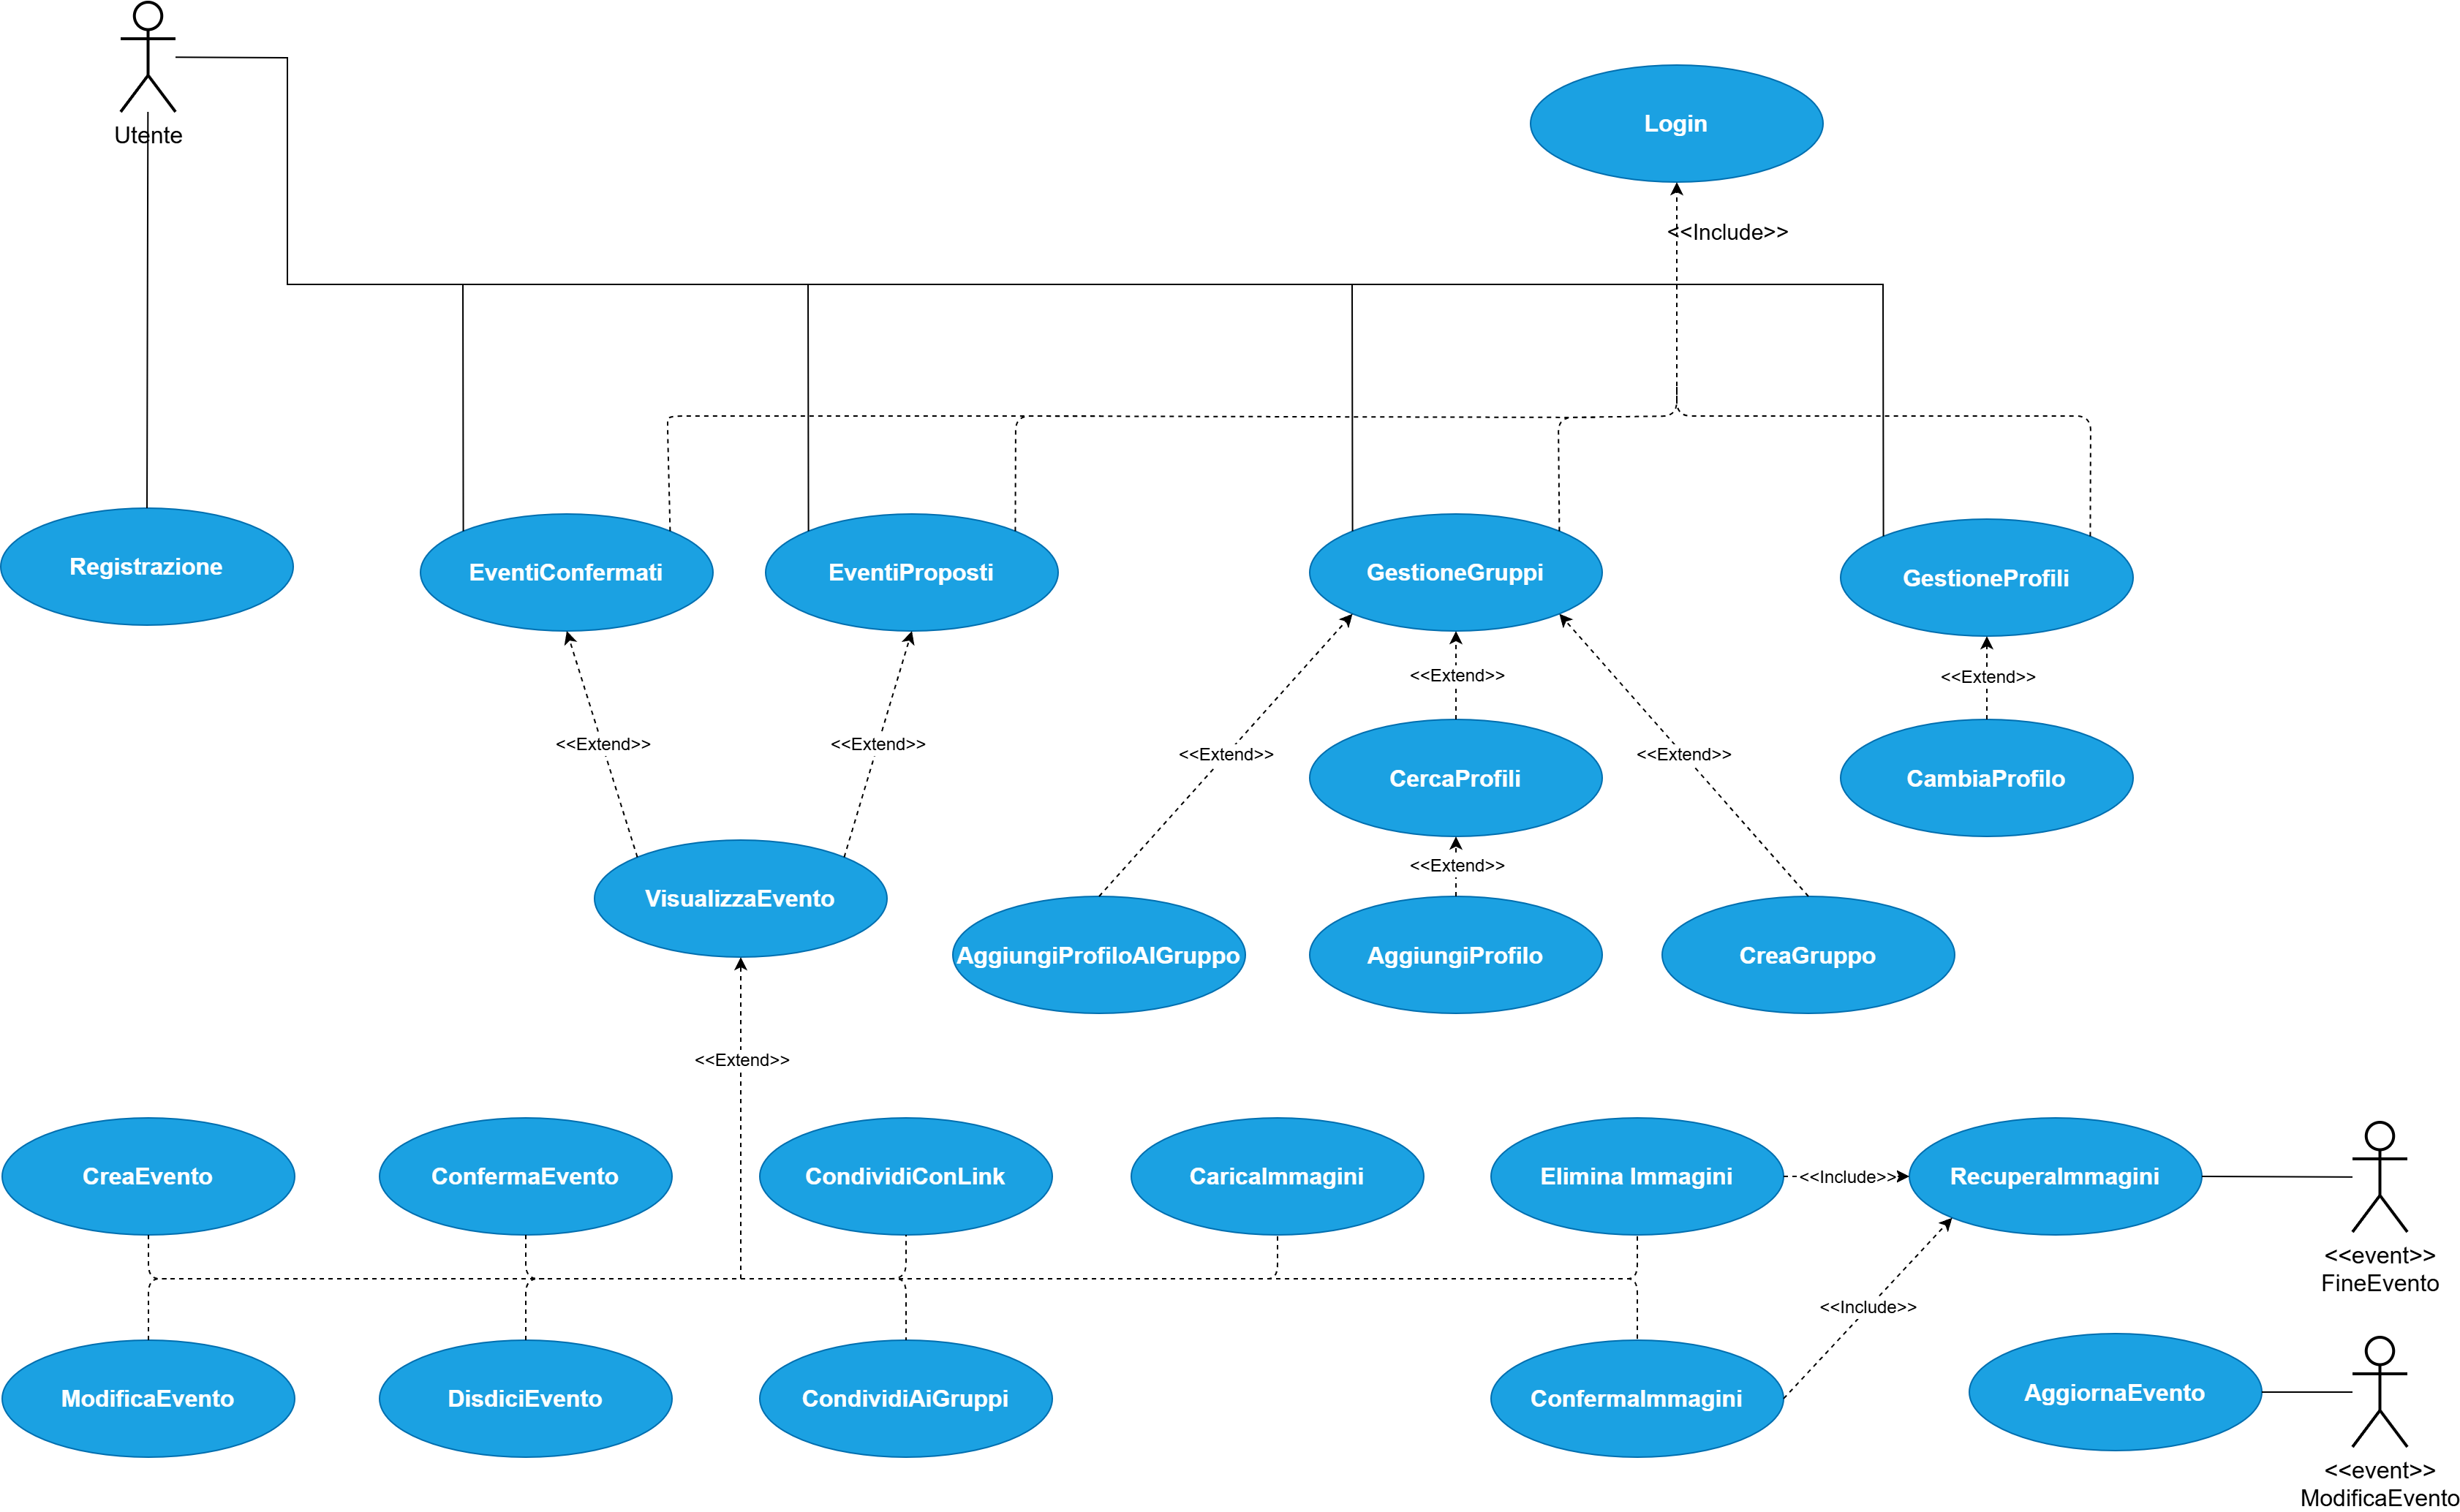
\includegraphics{Casiduso.png}}
    \caption{Diagramma dei casi d'uso}
\end{figure}

per ogni caso d'uso si identifica uno scenaro di utilizzo, che descrive le particolarità, le aspettative e i punti critici dell'utilizzo.
In particolare, si riportano gli scenari di utilizzo per i casi d'uso principali.
\clearpage
Lo scenario di registrazione vede la responsabilità, oltre che di creare un account, di associare un profilo all'utente.
Questo permette di avere una struttura gerarchica che permette di associare più profili ad un'unico utente, che può in seguito crearne di nuovi.\\

\begin{table}[htb]
    \begin{tabular} {|P{4.5cm}|P{11cm}|}
        \hline
        \textbf{Titolo}                   & Registrazione                                                                         \\
        \hline
        \textbf{Descrizione}              & L'utente si registra al servizio                                                      \\
        \hline
        \textbf{Attori}                   & Utente                                                                                \\
        \hline
        \textbf{Relazioni}                &                                                                                       \\
        \hline
        \textbf{Precondizioni}            &                                                                                       \\
        \hline
        \textbf{Postcondizioni}           & L'utente è registrato nel sistema e può interagire con il resto dell'applicazione     \\
        \hline
        \textbf{Scenario principale}      & 1.L'utente accede alla schermata di registrazione      \newline
        2. L'utente inserisce email e  password                      \newline
        3. Il sistema crea un account con le credenziali inserite, associando un utente ed un primo profilo   \newline
        4. L'utente termina la registrazione, se avvenuta con successo viene reindirizzato alla pagina principale
        \\
        \hline
        \textbf{Scenari Alternativi}      &

        Il sistema verifica che è già presente un account con la mail inserita, quindi procede con la procedura di login normale. \\
        \hline
        \textbf{Requisiti non funzionali} &
        Per interagire l’utente deve essere autenticato \linebreak
        Velocità in lettura e scrittura dei dati                                                                                  \\
        \hline
        \textbf{Punti aperti}             &                                                                                       \\
        \hline
    \end{tabular}

    \caption{Scenario di registrazione}
\end{table}

\clearpage

A seguito della modifica dell'evento, oltre al salvataggio dei dati, viene chiesto l'aggiornamento in tempo reale di tutte le parti interessate.
La modifica dei dati comporta inoltre un controllo sulle richieste contemporanee per evitare conflitti.\\
\begin{table}[htb]
    \begin{tabular} {|P{4.5cm}|P{11cm}|}
        \hline
        \textbf{Titolo}                   & ModificaEvento                                                                               \\
        \hline
        \textbf{Descrizione}              & Salva le modifiche ad un evento                                                              \\
        \hline
        \textbf{Attori}                   & Utente                                                                                       \\
        \hline
        \textbf{Relazioni}                & VisualizzaEvento                                                                             \\
        \hline
        \textbf{Precondizioni}            & L'evento esiste e sono stati modificati dei dati                                             \\
        \hline
        \textbf{Postcondizioni}           & Le modifiche vengono salvate e propagate a tutti i profili collegati                         \\
        \hline
        \textbf{Scenario Principale}      & 1. VisualizzaEvento \linebreak
        2. Il sistema controlla che i dati modificati siano corretti\linebreak
        3. I cambiamenti vengono salvati\linebreak
        4. Tutti i dispositivi collegati ai profili collegati all'evento visualizzano le immagini                                        \\
        \hline
        \textbf{Scenari Alternativi}      & 2. Se i dati risultano sbagliati, il sistema notifica l'utente originario indicando l'errore \\
        \hline
        \textbf{Requisiti non funzionali} & Velocità in lettura e scrittura dei dati \newline
        Scalabilità delle richieste                                                                                                      \\
        \hline
        \textbf{Punti aperti}             & Le modifiche all'evento devono essere consistenti, anche in caso di richieste simultanee     \\
        \hline
    \end{tabular}
    \caption{Scenario della modifica di un evento}
\end{table}

Il caricamento delle immagini è un'operazione di particolare importanza vista la sua importanza
nel coinvolgimento degli utenti alle funzionalità centrali dell'applicazione, e quindi al successo del progetto.
Olte a mostrare un'interfaccia intuitiva, il sistema deve essere in grado di gestire le richieste di caricamento in modo efficiente e scalabile.\\
\clearpage

\begin{table}[htb]
    \begin{tabular} {|P{4.5cm}|P{11cm}|}
        \hline
        \textbf{Titolo}                   & CaricaImmagini                                                                  \\
        \hline
        \textbf{Descrizione}              & Permette all'utente di selezionare immagini da collegare all'evento, salvandole \\
        \hline
        \textbf{Attori}                   & Utente                                                                          \\
        \hline
        \textbf{Relazioni}                & VisualizzaEvento                                                                \\
        \hline
        \textbf{Precondizioni}            & L'evento esiste                                                                 \\
        \hline
        \textbf{Postcondizioni}           & Le immagini vengono salvate e propagate a tutti i profili collegati             \\
        \hline
        \textbf{Scenario Principale}      & 1. VisualizzaEvento \linebreak
        2. L'utente seleziona le immagini che vuole caricare\linebreak
        3. Le immagini vengono salvate\linebreak
        4. Tutti i dispositivi relativi ai profili collegati all'evento visualizzano le immagini                            \\
        \hline
        \textbf{Scenari Alternativi}      &
        Scenario alternativo A:\linebreak
        3. Almeno una delle immagini crea problemi di lettura,
        l'utente viene notificato e può riprovare a caricare le immagini\newline
        Scenario alternativo B:\newline
        3. Solo una parte delle immagini vengono salvate, altre comportano errori\newline
        4. l'utente viene notificato dell'errore e può riprovare a caricare le immagini\newline
        5. Tutti i dispositivi relativi ai profili collegati all'evento visualizzano le immagini\newline
        Scenario alternativo C:\linebreak
        3. Nessuna immagine risulta salvata con successo\linebreak
        4. l'utente viene notificato dell'errore e può riprovare a caricare le immagini                                     \\
        \hline
        \textbf{Requisiti non funzionali} & Semplicità e fluidità dell'interfaccia grafica   \linebreak
        Velocità in lettura e scrittura dei dati\linebreak
        Scalabilità delle richieste                                                                                         \\
        \hline
        \textbf{Punti aperti}             &                                                                                 \\
        \hline
    \end{tabular}

    \caption{Scenario del caricamento delle immagini}
\end{table}
\clearpage

L'azione di recupero delle immagini semplifica l'utilizzo dell'applicazione, spostando l'azione richiesta all'utente dalla ricerca delle immagini alla sola conferma.
La sua corretta implementazione ne fa apprezzare l'utilità, con un significativo impatto sull'esperienza utente.\\

\begin{table}[htb]
    \begin{tabular} {|P{4.5cm}|P{11cm}|}
        \hline
        \textbf{Titolo}                   & RecuperaImmagini                                                                                                                           \\
        \hline
        \textbf{Descrizione}              & L'applicazione controlla la galleria e salva in locale le foto scattate durante l'evento                                                   \\
        \hline
        \textbf{Attori}                   & FineEvento                                                                                                                                 \\
        \hline
        \textbf{Relazioni}                & EliminaImmagini, ConfermaImmagini                                                                                                          \\
        \hline
        \textbf{Precondizioni}            & L'evento esiste ed è concluso\linebreak
        l'utente ha dato il permesso all'accesso alla galleria                                                                                                                         \\
        \hline
        \textbf{Postcondizioni}           & Le immagini sono salvate in locale e l'utente viene notificato                                                                             \\
        \hline
        \textbf{Scenario Principale}      & 1. Il sistema attende la fine dell'evento\linebreak
        2. Il sistema controlla la galleria per trovare le immagini scattate nell'arco temporale dell'evento\linebreak
        3. Se ci sono immagini, vengono salvate in locale e l'utente viene notificato                                                                                                  \\
        \hline
        \textbf{Scenari Alternativi}      &                                                                                                                                            \\
        \hline
        \textbf{Requisiti non funzionali} & Velocità in lettura e scrittura dei dati                                                                                                   \\
        \hline
        \textbf{Punti aperti}             & L'implementazione dipende dal dispositivo su cui viene eseguita l'applicazione, alcuni dispositivi potrebbero non permetterne l'esecuzione \\
        \hline
    \end{tabular}


    \caption{Scenario di recupero delle immagini dal dispositivo dell'utente}
\end{table}

\clearpage
\subsubsection{I requisiti di sicurezza}

Per definire i requisiti di sicurezza è prima richiesta un'analisi del rischio.
L'analisi del rischio avviene partendo dalla valutazione dei beni, dall'identificazione delle minacce e dei punti deboli noti,
per individuare i possibili vettori di attacco e concentrare le risorse dove più necessario.

\begin{table}[htb]

    \begin{tabular} {|P{3.5cm}|P{5.5cm}|P{6.7cm}|}
        \hline
        \textbf{Bene}                     & \textbf{Valore}                                                                                              & \textbf{Esposizione}      \\
        \hline
        Sistema Informativo               & Alto. Fondamentale per il funzionamento del servizio                                                         &
        Alta. Perdita finanziaria e di immagine                                                                                                                                      \\
        \hline
        Informazioni dei clienti          & Alto. Informazioni personali                                                                                 &
        Alta. Perdita di immagine dovuta alla divulgazione
        di dati sensibili                                                                                                                                                            \\
        \hline
        Informazioni relativi agli eventi & Medio-alto, necessari per offrire il servizio e contenenti informazioni personali e potenzialmente riservate &
        Molto Alta. Perdita di immagine possibile con la divulgazione dei dati relativi ai
        clienti                                                                                                                                                                      \\
        \hline
        Dati dei gruppi                   & Medio. Necessario per condividere gli eventi                                                                 & Alta. Perdita di immagine \\
        \hline
    \end{tabular}
    \caption{Valutazione dei beni}
\end{table}

\begin{table}[htbp]
    \centering
    \begin{tabular} {|P{3cm}|P{2cm}|P{6.1cm}|P{4cm}|}
        \hline
        \textbf{Minaccia}                                 & \textbf{Probab.} & \textbf{Controllo}                                                                                                                                                                                                                      & \textbf{Fattibilità}                                              \\
        \hline
        Furto credenziali utente                          & Alta             & Controllo sulla sicurezza della password - Log delle operazioni, autenticazione a due fattori                                                                                                                                           & Costo implementativo medio                                        \\
        \hline
        Alterazione o intercettazione delle comunicazioni & Alta             & Utilizzo di un canale sicuro - Log delle operazioni, autenticazione integrata nel messaggio                                                                                                                                             & Basso costo di realizzazione con determinati protocolli           \\
        \hline
        Accesso non autorizzato al database               & Bassa            & Accesso da macchine sicure - Log di tutte le operazioni                                                                                                                                                                                 & Basso costo di realizzazione, il server deve essere ben custodito \\
        \hline
        DoS                                               & Bassa            & Controllo e limitazione delle richieste                                                                                                                                                                                                 & Media complessità di implementazione                              \\
        \hline
        Saturazione del database                          & Bassa            & 1. Limitazione delle richieste in un dato intervallo di tempo. \linebreak 2. Limitazione della grandezza delle richieste singole \linebreak 3. Limitazione della grandezza richiesta dallo stesso utente in un dato intervallo di tempo & Media complessità di implementazione                              \\
        \hline
    \end{tabular}

    \caption{Tabella delle minacce}
    \label{<label>}
\end{table}

\begin{table}[htbp]
    \centering
    \begin{tabular} {|P{4cm}|P{12cm}|}
        \hline
        Tecnologia                     & Vulnerabilità                                            \\
        \hline
        Autenticazione email/password  & • Utente rivela volontariamente la password \linebreak
        • Utente rivela la password con un attacco di ingegneria sociale \linebreak
        • Password banali                                                                         \\
        \hline
        Cifratura comunicazioni        & • In caso di cifratura simmetrica particolare
        attenzione va alla lunghezza delle chiavi ed alla loro memorizzazione                     \\
        \hline
        Architettura Client/Server     & • DoS \linebreak
        • Man in the Middle \linebreak
        • Sniffing delle comunicazioni                                                            \\
        \hline
        Connessione Server/Persistenza & • Limite massimo di connessioni contemporanee \linebreak
        • Saturazione del Database                                                                \\
        \hline
    \end{tabular}
    \caption{Analisi tecnologica della sicurezza}
    \label{<label>}
\end{table}

\clearpage
Si prevedono quindi i principali attori malevoli e i relativi casi d'uso, per poi definire i requisiti su cui si baseranno le contromisure necessarie.
\begin{figure}[h!]
    \begin{center}
        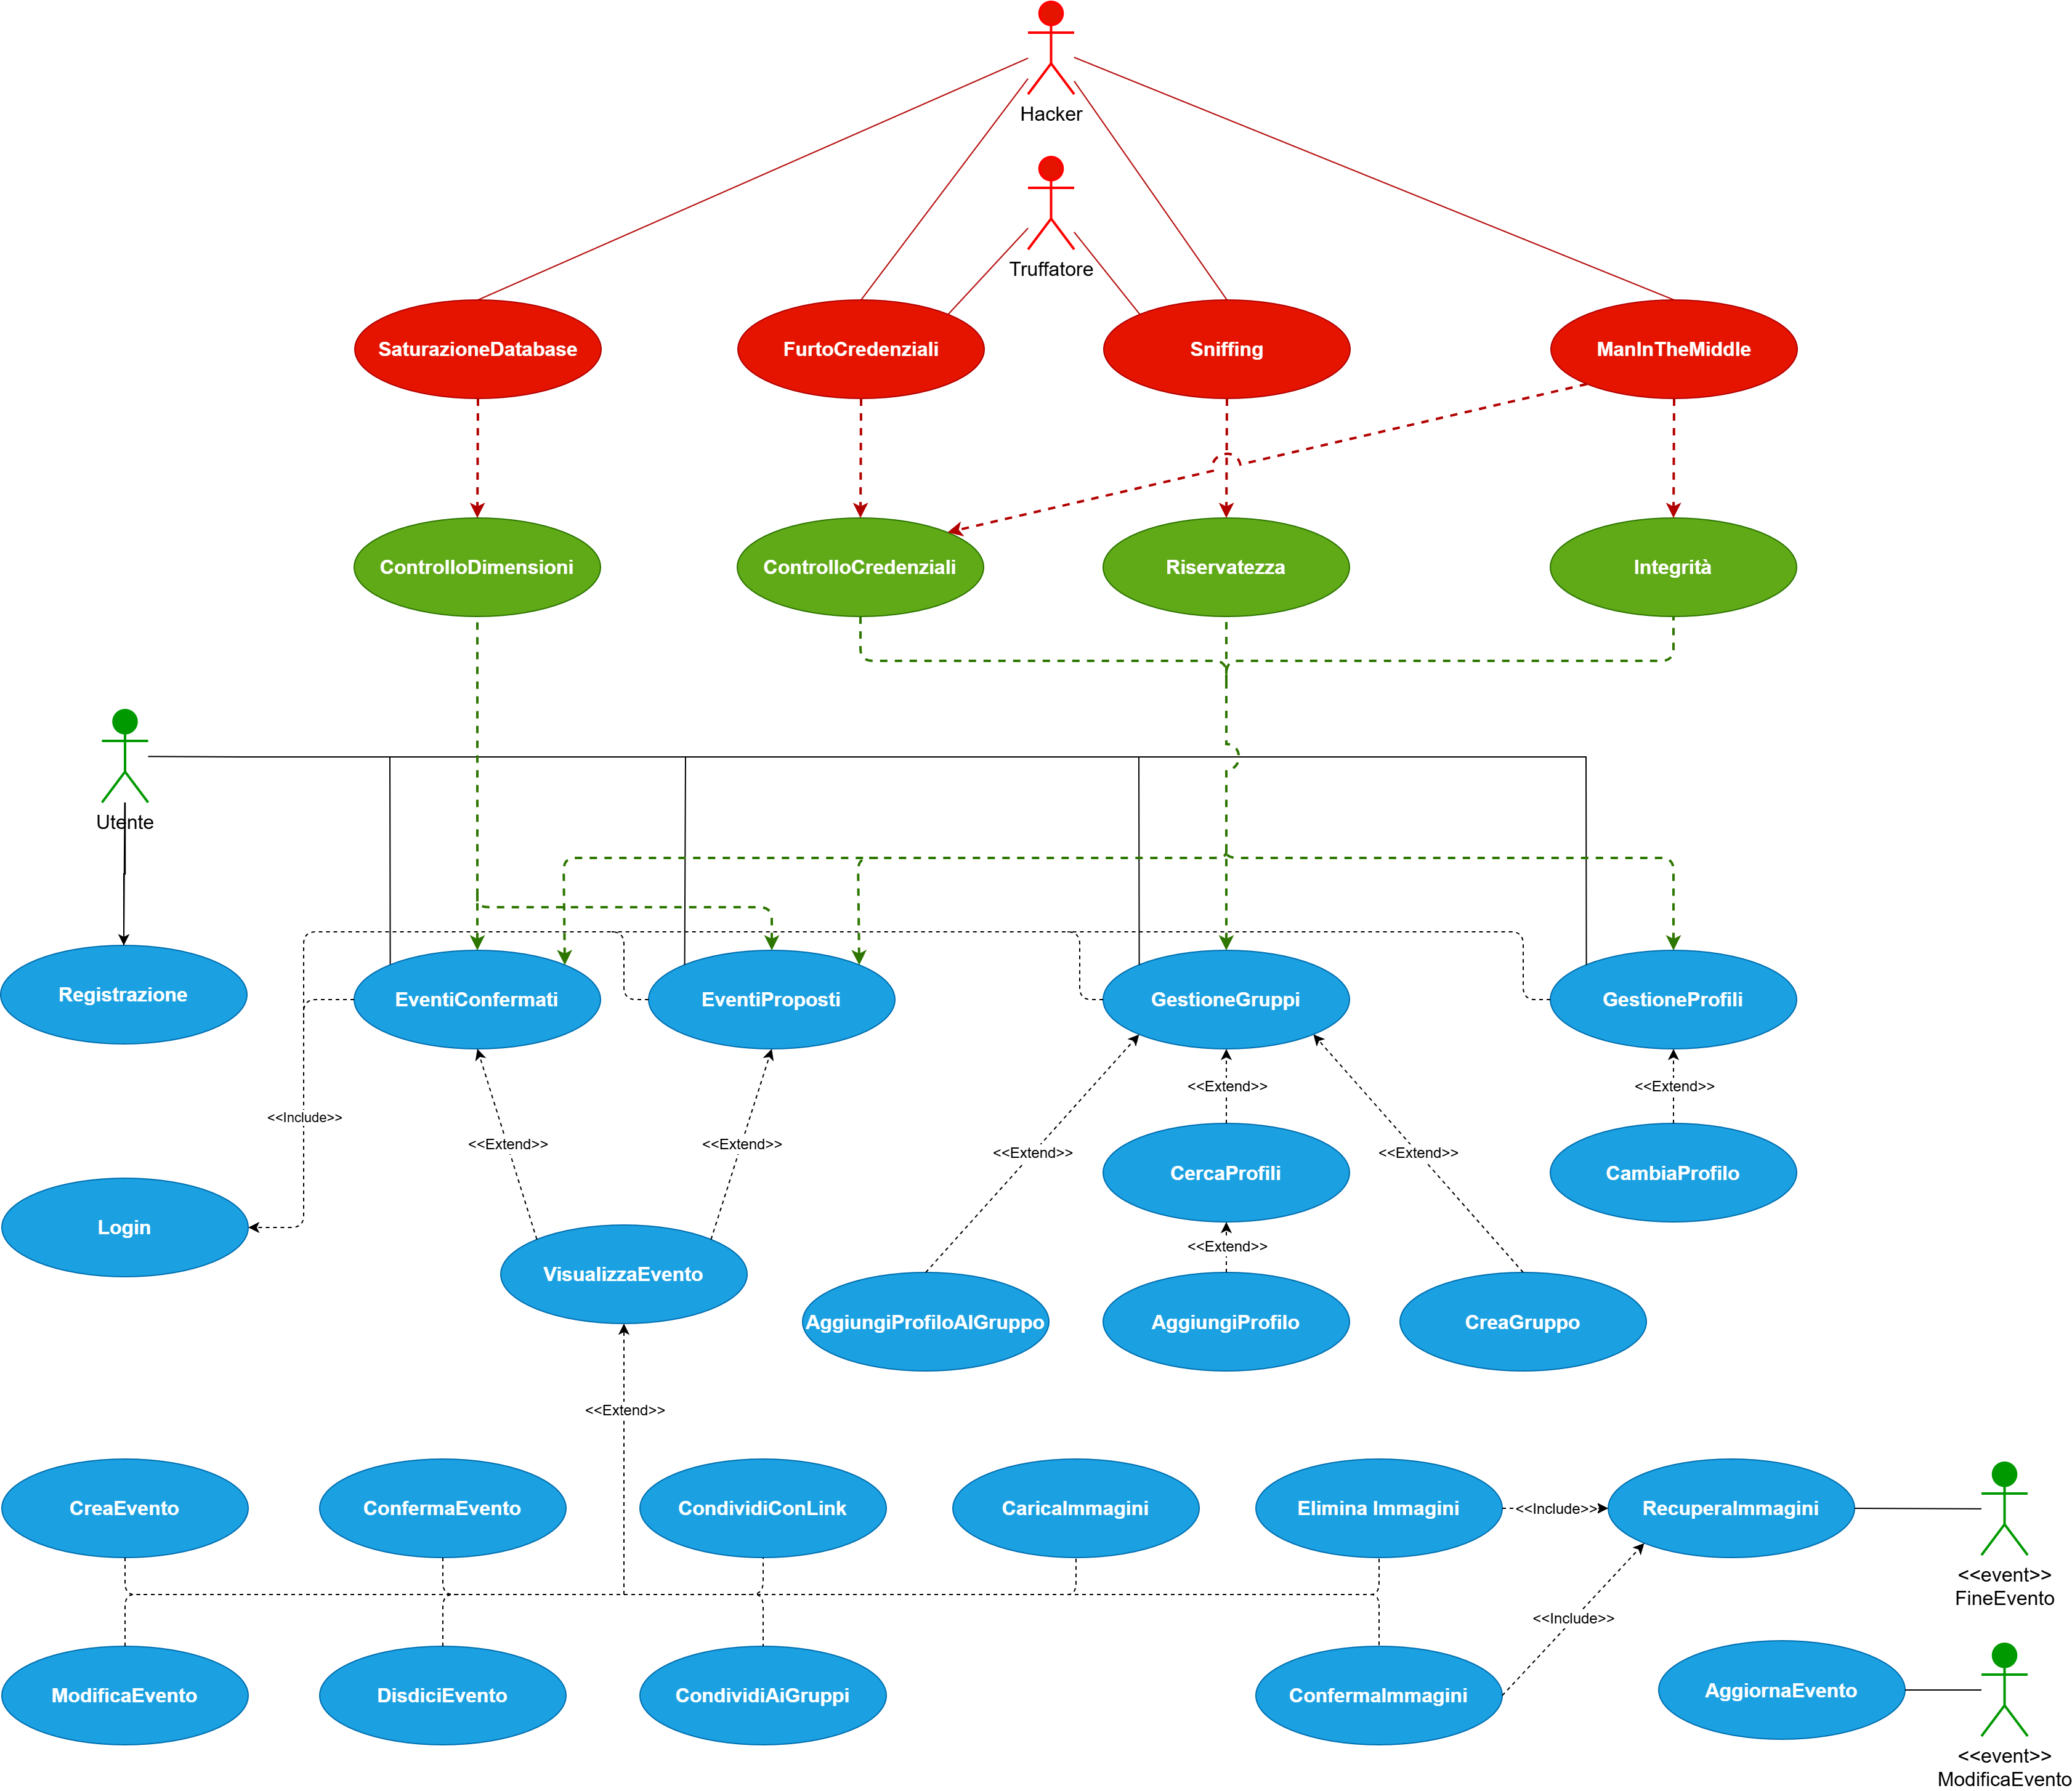
\includegraphics[width=\textwidth]{SecurityCase.png}
        \caption{Casi d'uso relativi alla sicurezza}
    \end{center}

\end{figure}
\clearpage

Sussistono quindi i seguenti requisiti inerenti alla protezione dei dati:
\begin{enumerate}
    \item Implementare un sistema di log per tracciare tutti i messaggi tra i client e i server, inclusi gli accessi, le richieste di prenotazione, di conferma, di sospensione e di invio e ricezione di dati
    \item I dati salvati devono essere protetti da un attaccante che abbia accesso al sistema, prendendo misure di sicurezza fisica, eventualmente cifrando i dati
    \item I dati inviati tra le parti remote devono essere protetti, utilizzando la cifratura dei dati
    \item Tutte le azioni avvenute sul sistema devono essere tracciate tramite un sistema di log.
\end{enumerate}

La visione e l'analisi dei log verrà gestita con uno strumento esterno, accessibile solo al personale autorizzato.


\begin{table}[htbp]
    \centering
    \begin{tabular} {|P{1.3cm}|P{11.2cm}|P{3cm}|}
        \hline
        \textbf{ID}                       & \textbf{Requisiti}                                                  & \textbf{Tipo} \\
        \hline
        R21F                              & Implementazione di un sistema di log per tracciare tutti i messaggi
        tra i client e i server           & Funzionale                                                                          \\
        \hline
        R22F                              & Le richieste non devono superare una certa dimensione               & Funzionale    \\
        \hline
        R7NF                              & I dati salvati devono essere protetti da un attaccante che abbia
        accesso al sistema, prendendo misure di sicurezza fisica, eventualmente
        cifrando i dati                   & Non Funzionale                                                                      \\
        \hline
        R8NF                              & I dati inviati tra le parti remote devono essere protetti, utilizzando la cifratura dei dati & Non Funzionale                                                                      \\
        \hline
    \end{tabular}
    \caption{Requisiti di sicurezza}
\end{table}

\clearpage